\documentclass{article}
\usepackage{tikz}
\begin{document}

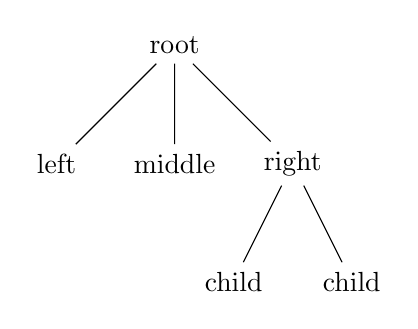
\begin{tikzpicture}
\node {root}
    child {
    node {left}
    }
    child{ node{middle}}
    child {
    node {right}
    child {node {child}}
    child {node {child}}
    };
\end{tikzpicture}

% \begin{tikzpicture}
% [edge from parent fork down, sibling distance=15mm, level distance=15mm,
% every node/.style={fill=red!30,rounded corners},
% edge from parent/.style={red,-o,thick,draw}]
% \node {root}
% child {node {left}}
% child {node {right}
% child {node {child}}
% child {node {child}}
% };
% \end{tikzpicture}
\end{document}
%%% Local Variables:
%%% mode: latex
%%% TeX-master: t
%%% End:
